\chapter{Solução e Avaliação da Proposta}
\section{Solução Proposta}

%TODO: Inserir figura.
A solução proposta nesse trabalho de conclusão de curso é o projeto de um carregador
\textit{onboard} trifásico que seja projetado para operar na rede elétrica presente nas
principais cidades brasileiras, com tensão de fase de \(127\ V_\mathrm{rms}\). A primeira etapa
do trabalho consiste no projeto de um retificador trifásico PFC em ponte completa visto na
figura e seu respectivo sistema de controle. A segunda etapa é relativa ao estudo teórico e
projeto do conversor \textit{Phase Shifted Full Bridge} e do conversor \textit{Dual Active
    Bridge}. O objetivo é comparar os dois conversores em termos de desempenho e complexidade de
projeto. Ademais, o DAB é também projetado para obter um carregador elétrico bidirecional.

Conforme a Figura \ref{fig:controlepfc3ph}, o controle do PFC trifásico apresenta uma malha
externa de tensão, que compara a tensão de saída do retificador com uma referência de tensão
CC. A saída do controlador de tensão é utilizada como referência para a componente de eixo
direto da corrente, enquanto que a referência da corrente em quadratura é nula, para garantir o
fator de potência unitário.

\begin{figure}
    \centering
    \caption{Esquema de controle do PFC trifásico.}
    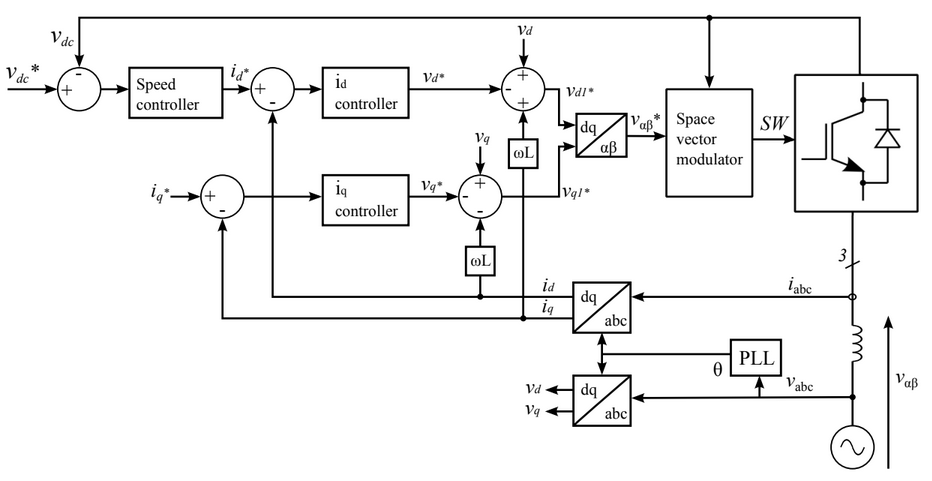
\includegraphics[width=0.8\textwidth]{./Figuras/controlepfc3ph.png}
    \legend{Fonte: \cite{3phPlecs}.}
    \label{fig:controlepfc3ph}
\end{figure}

\section{Avaliação da Solução}
Esta seção deve conter uma explicação de como será feita a avaliação da solução uma vez que ela
estiver concluída. O método de avaliação é dependente do projeto e o seu orientador pode
guiá-lo para a forma de avaliação mais adequada.
